\documentclass[a4paper,11pt]{article}

\usepackage[left=1cm,top=1cm]{geometry}
\usepackage[czech]{babel}
\usepackage[utf8]{inputenc}
\usepackage{helvet}
\renewcommand{\familydefault}{\sfdefault}

\usepackage{graphicx} % photo
\usepackage{paracol} % two columns
\usepackage{parcolumns}
\usepackage{xcolor} %colors
\usepackage{hyperref}

\begin{document}
\setlength{\parindent}{0pt}
\thispagestyle{empty}

\columnratio{0.2,0.8}
\begin{paracol}{2}
\setlength{\columnseprule}{0.2pt}
\setlength{\columnsep}{1.5cm}
    \begin{leftcolumn}

        %%--- Photo
        \begin{figure}[h]
        \centering
        \fbox{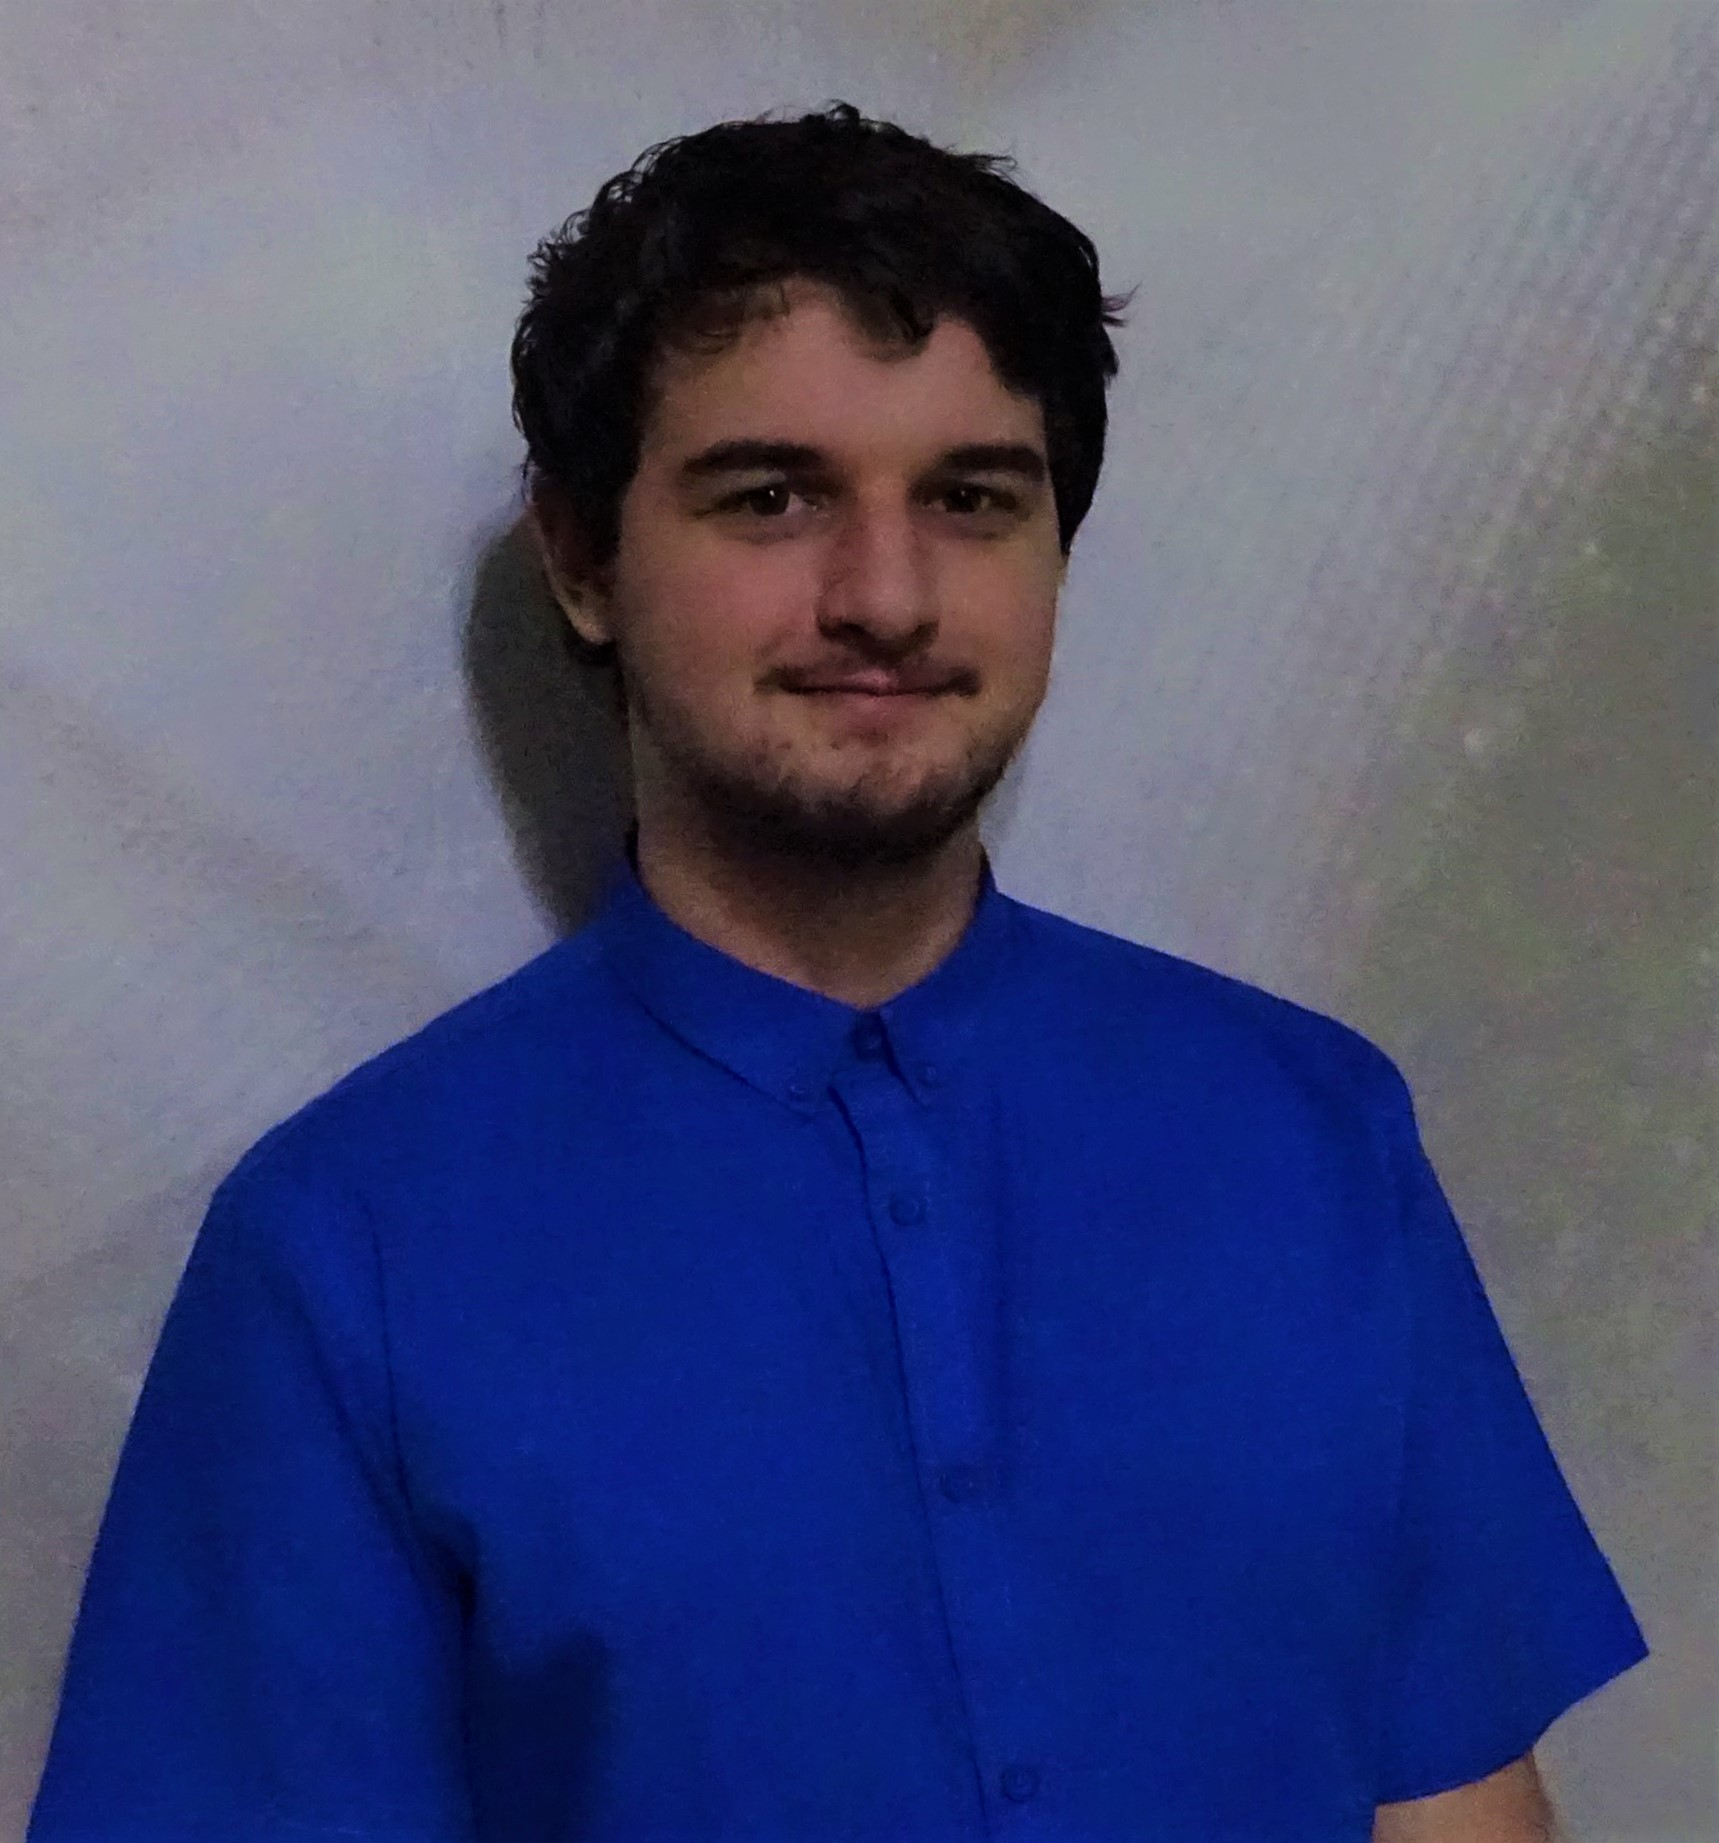
\includegraphics[width=1\linewidth]{Photo.jpg}}
        \end{figure}

        %%--- CAPTIONS
        \begin{flushright}
          \textbf{Praxe} \\
          \vspace{66pt}
          \textbf{Vzdělání} \\
          \vspace{120pt}
          \textbf{Znalosti} \\
          \vspace{86pt}
          \textbf{GitHub} \\
          \vspace{20pt}
          \textbf{Jazyky} \\
          \vspace{30pt}
          \textbf{Licence} \\
          \vspace{45pt}
          \textbf{Zájmy}



        \end{flushright}

    \end{leftcolumn}

    \begin{rightcolumn}

      %%--- BASIC INFORMATION
        \vspace*{1pt}
        \qquad{\LARGE\textbf{Adam Buchta}} \vspace{0.5cm} \\
        \hspace*{0.5cm} 
\includegraphics[width=0.3cm]{phone.png}~~+420 732 343 981 \hfill 
\includegraphics[width=0.3cm]{email.png}~~adbuch7@gmail.com \hspace*{2cm} \vspace{0.4cm} \\
        \hspace*{0.5cm} 
\includegraphics[width=0.3cm]{person.png}~~7.2.1998 \hfill 
\includegraphics[width=0.3cm]{house.png}~~Brno, Česká republika   \hspace*{2cm} \vspace{8pt} \\
        \rule{\linewidth}{0.5pt}

      %%--- CAREER
        \vspace{32pt}
        \begin{parcolumns}[colwidths={1=0.3\textwidth}]{2}
        \colchunk{ Tři týdny v roce 2017 }
        \colchunk{Red Hat, Inc. \\
                    \textcolor{gray}{Stážista. Školní praxe.}}
        \end{parcolumns}

        \vspace{5pt}
        \begin{parcolumns}[colwidths={1=0.3\textwidth}]{2}
        \colchunk{ 2011 - 2018 }
        \colchunk{Šálek Ticha, s.z. \\
                   \textcolor{gray}{Obsluha v čajovně.} }
        \end{parcolumns}



      %%--- EDUCATION
        \vspace{18pt}
        \begin{parcolumns}[colwidths={1=0.3\textwidth}]{2}
        \colchunk{ 2018 - 2019 }
        \colchunk{Vysoké učení technické v Brně, fakulta informačních technologií. \\
                    \textcolor{gray}{Tři semestry. Studium ukončeno.}}
        \end{parcolumns}

        \vspace{5pt}
        \begin{parcolumns}[colwidths={1=0.3\textwidth}]{2}
        \colchunk{ 2014 - 2018 }
        \colchunk{Obchodní akademie Veselí nad Moravou - Informační a komunikační technologie. \\
                   \textcolor{gray}{SŠ s maturitou.} }
        \end{parcolumns}
        \vspace{0.5cm}
        \rule{\linewidth}{0.5pt}

      %%--- SKILLS
        \vspace{18pt}
        \begin{parcolumns}{2}
        \colchunk{C/C++ \qquad 
\includegraphics[width=0.4cm]{fullstar.png} 
\includegraphics[width=0.4cm]{fullstar.png} 
\includegraphics[width=0.4cm]{fullstar.png} 
\includegraphics[width=0.4cm]{estar.png} 
\includegraphics[width=0.4cm]{estar.png} \\
                   C\#  \hspace{36.5pt} 
\includegraphics[width=0.4cm]{fullstar.png} 
\includegraphics[width=0.4cm]{estar.png} 
\includegraphics[width=0.4cm]{estar.png} 
\includegraphics[width=0.4cm]{estar.png} 
\includegraphics[width=0.4cm]{estar.png}
        }

        \colchunk{Java \qquad 
\includegraphics[width=0.4cm]{fullstar.png} 
\includegraphics[width=0.4cm]{fullstar.png} 
\includegraphics[width=0.4cm]{fullstar.png} 
\includegraphics[width=0.4cm]{estar.png} 
\includegraphics[width=0.4cm]{estar.png} \\
                  PHP \qquad 
\includegraphics[width=0.4cm]{fullstar.png} 
\includegraphics[width=0.4cm]{estar.png} 
\includegraphics[width=0.4cm]{estar.png} 
\includegraphics[width=0.4cm]{estar.png} 
\includegraphics[width=0.4cm]{estar.png}
        }
        \end{parcolumns}

        \vspace{0.5cm}
        \normalsize{Další znalosti: MS Office, Gimp, CorelDraw, \textbf{GIT}, \LaTeX, MS Visual Studio, Linux (Ubuntu), (X)HTML, CSS, Assemler}

      %%--- GitHub
        \vspace{26pt}
        Můj GitHub: \url{https://github.com/adbu21}
        
        
      %%--- LANGUAGES
        \vspace{19pt}
        \begin{parcolumns}{2}
        \colchunk{Anglický jazyk \qquad 
\includegraphics[width=0.4cm]{fullstar.png} 
\includegraphics[width=0.4cm]{fullstar.png} 
\includegraphics[width=0.4cm]{fullstar.png} 
\includegraphics[width=0.4cm]{fullstar.png} 
\includegraphics[width=0.4cm]{halfstar.png}}
        \colchunk{Německý jazyk \qquad 
\includegraphics[width=0.4cm]{fullstar.png} 
\includegraphics[width=0.4cm]{halfstar.png} 
\includegraphics[width=0.4cm]{estar.png} 
\includegraphics[width=0.4cm]{estar.png} 
\includegraphics[width=0.4cm]{estar.png}}
        \end{parcolumns}

      %%--- LICENCE
        \vspace{28pt}
        Řidičský průkaz \textbf{B} \\ \\
        \rule{\linewidth}{0.5pt}

      %%--- INTERESTS
        \vspace{18pt}
        Člen v šermířském a hereckém klubu Dračí Úsvit, s.z. od roku 2010. \\
        Vášnivý hráč počítačových her.\\
        Dobrovolník v testování DLC hry Kingdom Come: Deliverance pro Warhorse Studios.

    \end{rightcolumn}
\end{paracol}

\end{document} 